\chapter{Placement Algorithm}
\section{Theory}
{\bf \noindent  Definition 1:} \\
Considering $n$ nodes for a Vertical hierarchical node (Fig. 6) with $n$ representing the number of children, its height and the width are calculated with the following formulas: \\
\vspace{-0.5cm}
\begin{subequations}
\begin{align}
Height &= max(Height_{Node_1}, Height_{Node_2}, \hdots, Height_{Node_n})\\
Width  &= \sum_{k=1}^{n} Width_{Node_k} 
\end{align}
\end{subequations}
For a Horizontal hiearchical node, we have:
\vspace{-0.25cm}
\begin{subequations}
\begin{align}
Height &= \sum_{k=1}^{n} Height_{Node_k} \\
Width  &=  max(Width_{Node_1}, Width_{Node_2}, \hdots, Width_{Node_n})
\end{align}
\end{subequations}
{\bf \noindent  Definition 2:} \\
Each $Node_X$ has $m$ pairs (height, width) representing the size that it can take, unless if the node is preset. When a node is preset, it has a single size height/width defined by the designer:

\begin{algorithm}
\caption{Possible sizes}
\eIf{$Node_X$ is preset}{
  $Node_X: [(Height_{\textit{preset}}, W_{\textit{preset}})]$
}{
  $Node_X: [(Height_1, Width_1), (Height_2, Width_2),\hdots ,(Height_m, Width_m)]$\\
  with $m$, number of sizes\\  
}
\end{algorithm}
The algorithm evaluates all the possible sets if they can be accepted based on the tolerance margins parameter for the height and the width of the hierarchical node. It starts with the first possible sizes of each node:

\begin{algorithm}
Initial set:\\
\begin{equation}
  HierarchicalNode (Height_1, Width_1) = 
  \begin{pmatrix}
    Node_1(Height_1, Width_1)  \\
    Node_2(Height_1, Width_1)  \\
    \vdots            \\
    Node_n(Height_1, Width_1)  
  \end{pmatrix}
\end{equation}\\
\end{algorithm}
\vspace{-0.5cm}

Once this set of pairs height/width is processed, $Node_1$ considers then its second size $(Height_2, Width_2)$ until all its possible sizes are considered. Once the last size is reached for $Node_1$, $Node_2$ passes to its second size and $Node_1$ back to its first possible size and so on. The main algorithm is the following one:

\begin{algorithm}
\caption{Main Placement Algorithm}
{\bf Case:} Vertical Node \\
\For{i = 1:Number of sets}{\vspace{0.25cm}
  Determine $(Height_{max_i}, Height_{min_i}, Width_{i})^{(1)}$\vspace{0.25cm}\\
  \If{ $(Height_{max_i} - Height_{min_i}) <=$ \textit{Height tolerance}$^{(2)}$ } 
  {Accept size $(Height_{i}, Width_{i})$} 
 
}\vspace{0.25cm}

{\bf Case:} Horizontal Node \\
Same algorithm except for $(1)$ and $(2)$.\\
$(1)$: Determine $(Width_{max_i}, Width_{min_i}, Height_{i})$\\
$(2)$: $(Width_{max_i} - Width_{min_i}) <=$ \textit{Width tolerance}\vspace{0.25cm}
\end{algorithm}
\newpage
The total number of sets to be evaluated is: 
\vspace{-0.25cm}
\begin{equation}
\textit{Number of sets} =  (m_{Node_1} * m_{Node_2} * \hdots * m_{Node_n})\\
\end{equation}

The number of sets to consider may seem to grow at a fast rate but some considerations need to be taken into account. Inside of a slicing tree, it is very common to have several hierarchical nodes which implies that some sets will be filtered by the condition $(2)$ of the main placement algorithm (Algorithm 2) for not respecting the margin tolerances. Moreover, a hierarchical node can contain symmetries between its children nodes. It means that for 2 symmetrical nodes, only $m$ possible sizes will be considered instead of $m^2$. 

\section{Results}

\begin{figure}[h]
\begin{center}
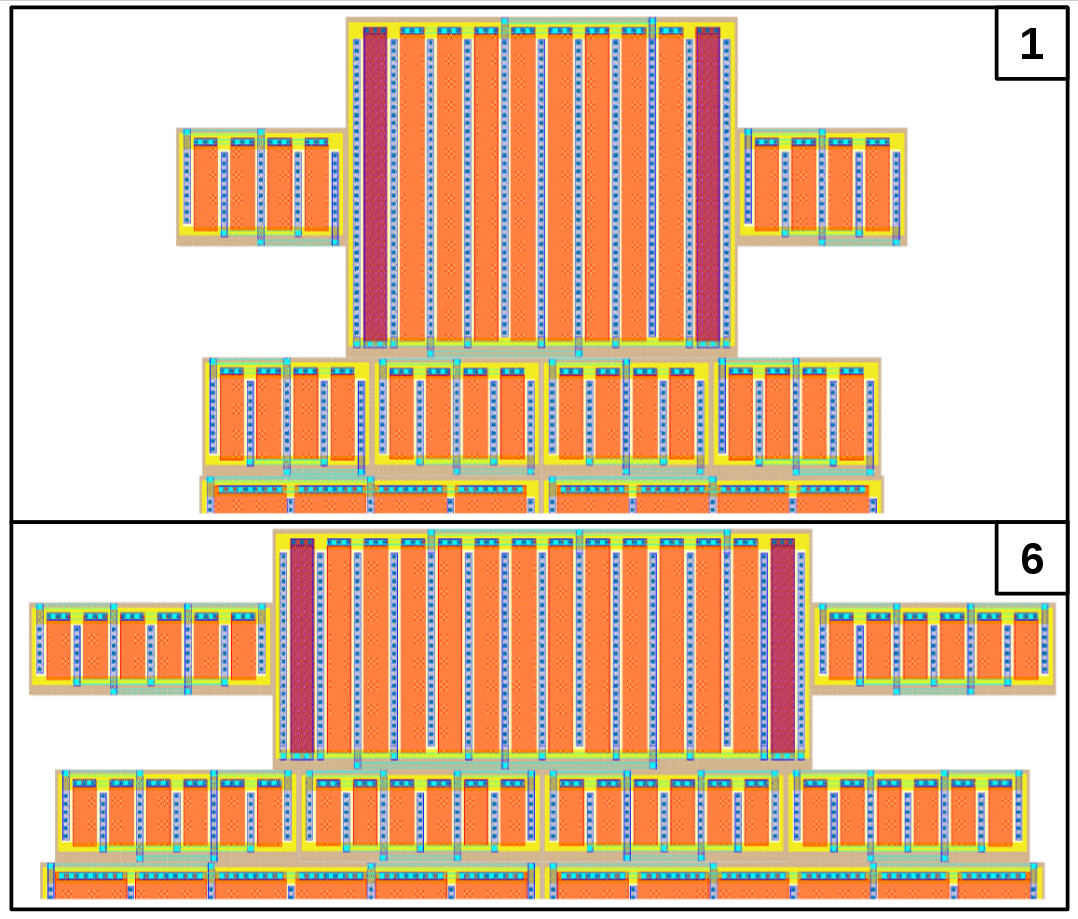
\includegraphics[width=80mm]{Figures/zoom.jpg}
\caption{Evolution of 2 rows from layout 1 and 6 of Table II for different global aspect ratios. These figures have the same scale.}
\end{center}
\end{figure}
\vspace{-0.5cm}

\begin{figure*}[t]
\begin{center}
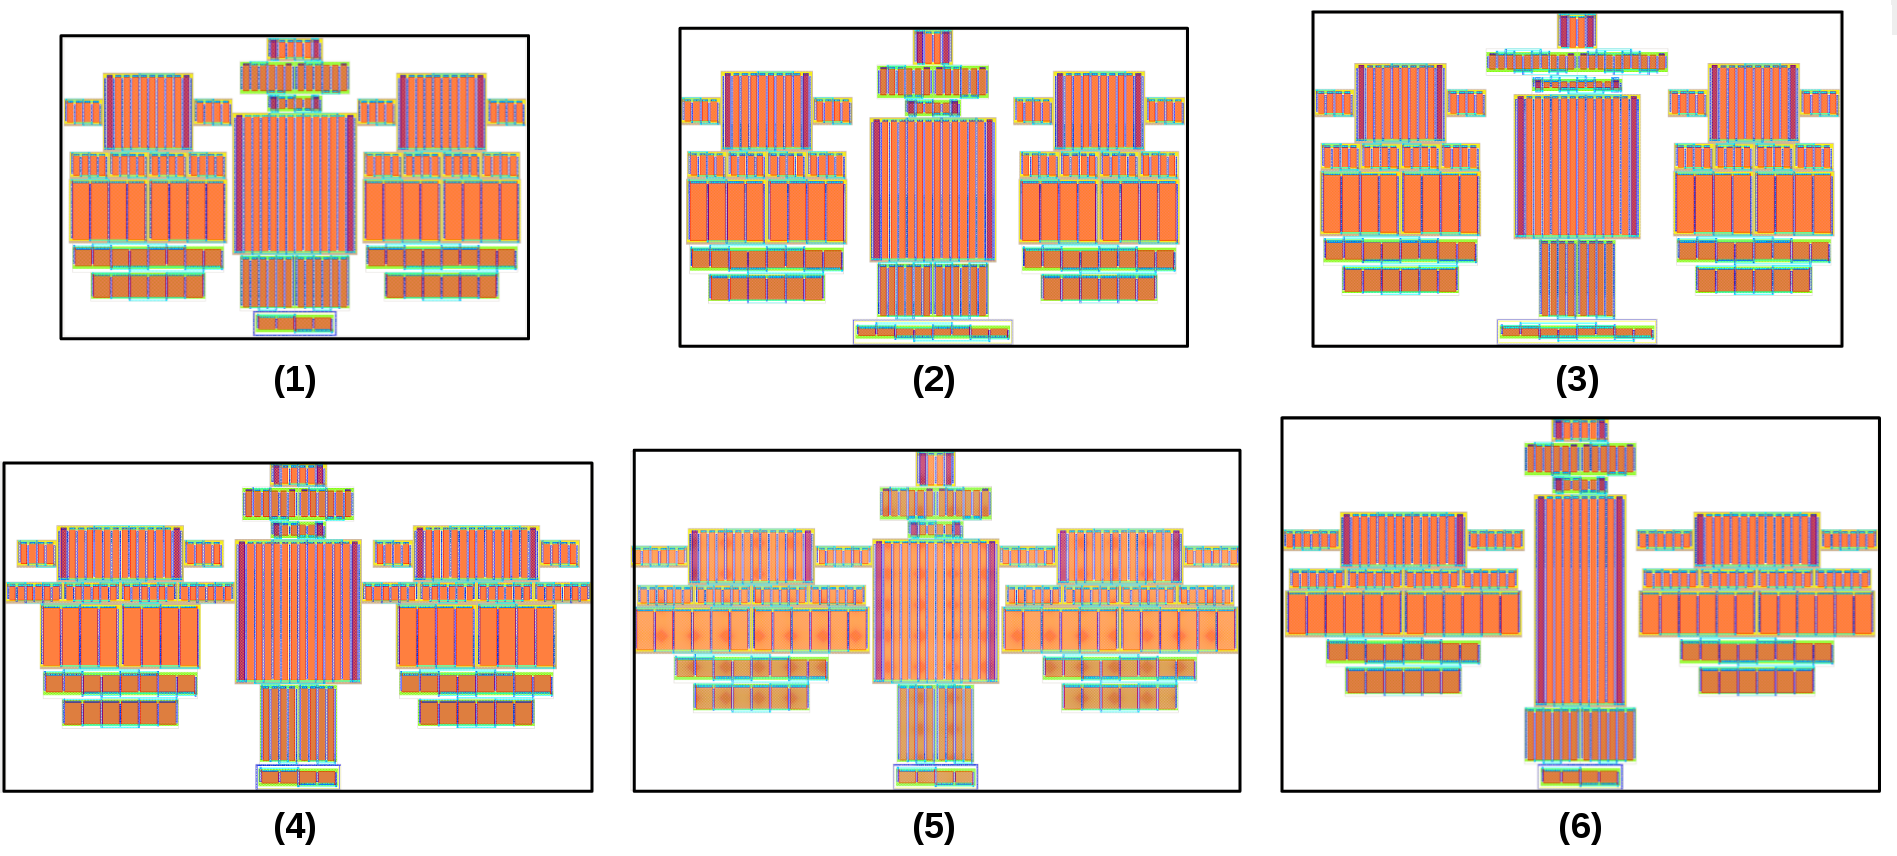
\includegraphics[width=150mm]{Figures/all.png}
\caption{Layouts of the fully differential transconductor cite{19} from Table II. These figures have all the same scale.}
\end{center}
\end{figure*}
Our placement algorithm was implemented in C++ programming language on a Intel(R) Core(TM) i5-4590S CPU @ 3.00 GHz workstation with 6 GB RAM. To illustrate the capability of our algorithm, we experiment it on a fully differential transconductor cite{19}, designed under a technology CMOS 130 nm.
\newline 
\newline 
\indent  The fully differential transconductor is composed of a total of 32 devices and we consider 2 possible variations for each device. The slicing tree takes into account 11 symmetries for this circuit and tolerance margins are set in a way to have reasonnable amount of accepted possibilities. Our algorithm found 384 possible placements in less than 1 second, some of them are listed on Table II and can be seen on Fig.8.
\newline 
\newline 
\indent  Table II shows the characteristics of those layouts with their total area, their width, their height and the percentage of the circuit occupation in the total area. Fig. 7  and Fig. 8 illustrate the layouts described in Table II and show the evolution of the rows for different global aspect ratios. The designer can choose his final placement based on his experience and preference. The placement results are plotted on a graph with heights and widths as axis and can be selected interactively to be placed in a few seconds.

\begin{table}[h]  
\caption{Some layout results of the fully differential transconductor}
\begin{minipage}{9cm}
\begin{tabular}{|C{2.5cm}|C{3cm}|C{3cm}|C{3cm}|C{2.5cm}|}
\hline
Layout & Area ($\mu m^2$) & Width ($\mu m$) & Height ($\mu m$) & Occupation ($\%$)\\
\hline
1 & 4600 & 84 & 54 & 68 \\
\hline
2 & 5116 & 91 & 57 & 63 \\
\hline
3 & 5603 & 94.2 & 59 & 58 \\
\hline
4 & 6162 & 105 & 59 & 52 \\
\hline
5 & 6648 & 109 & 61 & 49 \\
\hline
6 & 7105 & 107 & 67 & 46 \\
\hline
\end{tabular}
\end{minipage}
\end{table}